% Beamer presentation
\documentclass[11pt,aspectratio=43,ignorenonframetext,t]{beamer}

% Presentation settings
\mode<presentation>{
  \usetheme[framenumber,titleframestart=1]{UoM_alex}
  \usefonttheme{professionalfonts} % using non standard fonts for beamer
  \usefonttheme{serif}
  \usepackage{fontspec}
  \setmainfont[Ligatures=TeX]{Arial}
}

% Handout settings
\mode<article>{
  \usepackage{fullpage}
  \usepackage{fontspec}
  \setmainfont[Ligatures=TeX]{Arial}
  \setlength{\parskip}{1.5\baselineskip} % correct beamer line spacings
  \setlength{\parindent}{0cm}
  \usepackage{enumitem}
  \setlist[itemize]{topsep=0pt}
}

 % Packages
\usepackage{graphicx}
\graphicspath{{./images/png}} % generic graphics path; overridden if necessary
\usepackage{amsmath}
\allowdisplaybreaks[1] % allow eqnarrays to break across pages
\usepackage{amssymb} 
\usepackage[HTML]{xcolor}
\definecolor{uomlinkblue}{HTML}{0071BC}
\usepackage{hyperref}
\hypersetup{
  colorlinks=true,
  linkcolor=uomlinkblue,
  filecolor=uomlinkblue,      
  urlcolor=uomlinkblue,
  pdflang={en-GB},
}
\usepackage[document]{ragged2e} % left aligned text for accessibility
\usepackage{tikz}
\usetikzlibrary{positioning, arrows, arrows.meta}
\usepackage{unicode-math} % unicode maths for accessibility
\usepackage{pdfcomment}   % for alt text for accessibility
\usepackage{rotating}     % allow portrait figures and tables
\usepackage{subfigure}    % allow matrices of figures
\usepackage{float}        % allows H option on floats to force here placement
\usepackage{multirow}     % allows merging of rows in tables
\usepackage{tabularx}     % allows fixed width tables
\usepackage{ctable}       % modifies \hline for use in table
\usepackage{bm}           % allow bold fonts in equations
\usepackage{pgf}          % allow graphics manipulation
\usepackage{etoolbox}
  
% Custom commands
\newcolumntype{Z}{>{\centering\arraybackslash}X}  % tabularx centered columns 

\makeatletter
  \DeclareRobustCommand{\em}
  {
    \@nomath\em
    \if b
      \expandafter\@car\f@series\@nil \normalfont
    \else
      \bfseries
    \fi
  }
\makeatother

\makeatletter
  \preto{\@verbatim}{\topsep=0pt \partopsep=0pt}
\makeatother

\def\checkmark{
  \tikz\fill[scale=0.4](0,.35) -- (.25,0) -- (1,.7) -- (.25,.15) -- cycle;
}

% Counters
\newcounter{example_number} % keep track of the example questions

% Frontmatter
\newcommand{\cmclecture}[1]{
  \title{Combinatorial Mesh Calculus (CMC): Lecture #1}
}
\author{
  Lectured by:
  \href{https://scholar.google.com/citations?user=x4R-snQAAAAJ&hl=en}
  {Dr. Kiprian Berbatov}$^1$\\
  \smallskip
  Lecture Notes Compiled by:
  \href{https://scholar.google.com/citations?user=CoIpITkAAAAJ&hl=en}
  {Muhammad Azeem}$^1$\\
  \smallskip
  Under the supervision of:
  \href{https://scholar.google.co.uk/citations?user=3nWJe5wAAAAJ&hl=en}
  {Prof. Andrey P. Jivkov}$^1$\\
  \smallskip
  {\tiny $^1$Department of Mechanical and Aerospace Engineering,
    The University of Manchester, Oxford Road, Manchester M13 9PL, UK}
}

% Special frames
\newcommand{\cmctitleframe}{
  \titlepage
  \begin{tikzpicture}[remember picture,overlay]
    \node[anchor=south east] at (current page.south east) {
      \href{https://youtube.com/@kipi.berbatov}{
        \includegraphics[width=1.5cm]{youtube-icon.png}
      }
    };
  \end{tikzpicture}
}
\newcommand{\cmcendframe}{
  \begin{figure}
    \centering
    \includegraphics[width=0.85\linewidth]{Thanks.png}
  \end{figure}
}

\cmclecture{15}
\date{05 November 2025}

\usepackage{tikz}
\usetikzlibrary{calc}

\begin{document}

%========================= TITLE =========================
\begin{frame}
  \cmctitleframe
\end{frame}

\begin{frame}{Embeddability Caveat}
\begin{block}{Note}
A combinatorial mesh may embed into a manifold, yet its \emph{image} need not be a manifold (e.g., a vertex with three incident edges, or an edge shared by three faces).
\end{block}

\begin{columns}[t,onlytextwidth]
\column{0.48\textwidth}
\begin{center}
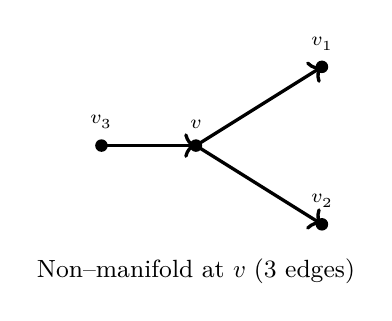
\begin{tikzpicture}[scale=1.0, dot/.style={circle,fill,inner sep=1.6pt}]
% Vertex with three incident edges (non-manifold vertex)
\coordinate (A) at (0,0);
\coordinate (B) at (1.6,1.0);
\coordinate (C) at (1.6,-1.0);
\coordinate (D) at (-1.2,0.0);

\node[dot,label= {$\scriptstyle v$}] at (A) {};
\node[dot,label= {$\scriptstyle v_1$}] at (B) {};
\node[dot,label= {$\scriptstyle v_2$}] at (C) {};
\node[dot,label= {$\scriptstyle v_3$}] at (D) {};

\draw[very thick,->] (A)--(B);
\draw[very thick,->] (A)--(C);
\draw[very thick,->] (D)--(A);

\node at (0,-1.6) {\small Non–manifold at $v$ (3 edges)};
\end{tikzpicture}
\end{center}

\column{0.52\textwidth}
\begin{center}
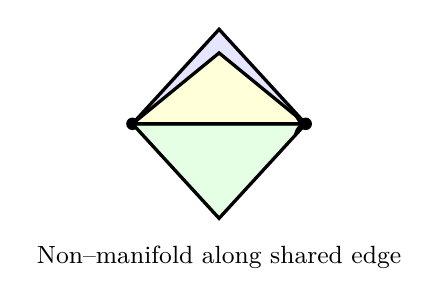
\begin{tikzpicture}[scale=1.0, dot/.style={circle,fill,inner sep=1.6pt}]
% One edge with three faces (non-manifold edge)
\coordinate (P0) at (0,0);
\coordinate (P1) at (2.2,0);
\coordinate (U) at (1.1,1.2);
\coordinate (D) at (1.1,-1.2);
\coordinate (W) at (1.1,0.9);

\node[dot] at (P0) {};
\node[dot] at (P1) {};

% three triangular faces sharing edge P0--P1
\fill[blue!10] (P0)--(U)--(P1)--cycle;
\fill[green!10] (P0)--(D)--(P1)--cycle;
\fill[yellow!15] (P0)--(W)--(P1)--cycle;

\draw[very thick] (P0)--(U)--(P1)--cycle;
\draw[very thick] (P0)--(D)--(P1)--cycle;
\draw[very thick] (P0)--(W)--(P1)--cycle;
\draw[very thick,->] (P0)--(P1);

\node at (1.1,-1.7) {\small Non–manifold along shared edge};
\end{tikzpicture}
\end{center}
\end{columns}
\end{frame}


\begin{frame}{Boundary and Interior Hyperfaces}
\vspace{-0.2cm}
\begin{block}{Property $(\ast)$}
Let a combinatorial mesh \(M\) with dimension \(D=\dim M\), graded by \(M=\bigcup_{p=0}^{D} M_p\) and face relation \(\preccurlyeq\) (``is a face of''). For any \((D\!-\!1)\)–cell \(c\in M_{D-1}\) define the set of incident top cells $\mathsf{Star}_D(c)\;:=\;\big\{\,a\in M_D \;\big|\; c\preccurlyeq a\,\big\},\ m(c)\;:=\; \big|\mathsf{Star}_D(c)\big|.$ We say that \(M\) satisfies \textbf{property $(\ast)$} iff every \((D\!-\!1)\)–cell has one or two incident \(D\)–cells: $\forall\,c\in M_{D-1}:\quad m(c)\in\{1,2\}.$

This induces the canonical classification of \((D\!-\!1)\)–cells: \textbf{Boundary hyperface:} $m(c)=1\ \Longleftrightarrow\; c$ belongs to exactly one $D$–cell; \textbf{Interior hyperface:} $m(c)=2\ \Longleftrightarrow\; c$ is shared by exactly two $D$–cells. We collect these as
\vspace{-0.3cm}
\begin{align*}
&\partial M\;:=\;\{\,c\in M_{D-1}\mid m(c)=1\,\},
\\ &\operatorname{int}_{D-1} M\;:=\;\{\,c\in M_{D-1}\mid m(c)=2\,\}.
\end{align*}

\end{block}
\end{frame}


\begin{frame}{Example 1: 1D Mesh}
\begin{block}{1D Mesh Example}
The mesh \(M\) consists of edges (1–cells) and vertices (0–cells).
Each vertex belongs to one or more edges:
\vspace{-0.3cm}
\begin{align*}
&\text{Endpoints (degree 1): Boundary nodes.}\\
&\text{Intermediate (degree ≥ 2): Interior nodes.}
\end{align*}
\end{block}

\begin{center}
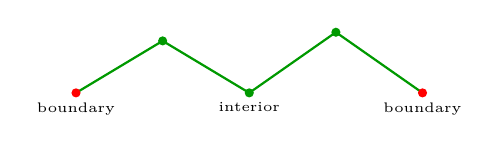
\begin{tikzpicture}[scale=1.1, dot/.style={circle,fill,inner sep=1.4pt}]
% nodes
\coordinate (A) at (0,0);
\coordinate (B) at (1,0.6);
\coordinate (C) at (2,0);
\coordinate (D) at (3,0.7);
\coordinate (E) at (4,0);

% edges
\draw[thick,green!60!black] (A)--(B)--(C)--(D)--(E);
% boundary
\fill[red] (A) circle (1.5pt);
\fill[red] (E) circle (1.5pt);
% interior
\foreach \p in {B,C,D}{\fill[green!60!black] (\p) circle (1.5pt);}
\node[below] at (A) {\tiny boundary};
\node[below] at (E) {\tiny boundary};
\node[below] at (C) {\tiny interior};
\end{tikzpicture}
\end{center}
\end{frame}


\begin{frame}{Example 2 - Pentagon Mesh (2D)}
\begin{columns}[t,onlytextwidth]
\column{0.55\textwidth}
\begin{block}{Interpretation}
In a 2D polygonal mesh, boundary edges belong to one face, while shared edges (if any) belong to two faces.
\end{block}

\column{0.45\textwidth}
\begin{center}
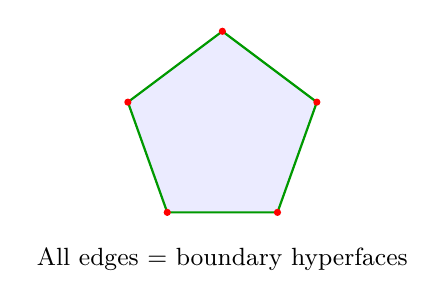
\begin{tikzpicture}[scale=1.0, dot/.style={circle,fill,inner sep=1.3pt}]
\coordinate (A) at (0,1.3);
\coordinate (B) at (1.2,0.4);
\coordinate (C) at (0.7,-1.0);
\coordinate (D) at (-0.7,-1.0);
\coordinate (E) at (-1.2,0.4);
\fill[blue!8] (A)--(B)--(C)--(D)--(E)--cycle;
\draw[thick,green!60!black] (A)--(B)--(C)--(D)--(E)--cycle;
% mark vertices
\foreach \p in {A,B,C,D,E}{\fill[red] (\p) circle (1.3pt);}
\node at (0,-1.6) {\small All edges = boundary hyperfaces};
\end{tikzpicture}
\end{center}
\end{columns}
\end{frame}

\begin{frame}{Example 3: Two Squares}
\begin{block}{Description}
Two faces \(F_1,F_2\) share one edge \(E_0\):
\vspace{-0.3cm}
\begin{align*}
& E_0 \text{ belongs to both } F_1,F_2\text{\ and } E_1 \text{\ belongs to }F_2\Rightarrow\ \text{interior}\\ & \text{hyperface.}\\
& \text{Other edges: each belongs to one face (boundary).}
\end{align*}
\end{block}

\begin{center}
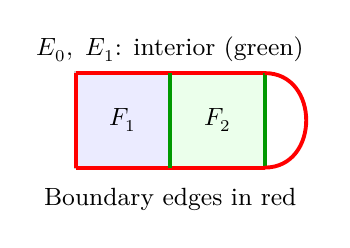
\begin{tikzpicture}[scale=1.0]
\fill[blue!8] (0,0)--(1.2,0)--(1.2,1.2)--(0,1.2)--cycle;
\fill[green!8] (1.2,0)--(2.4,0)--(2.4,1.2)--(1.2,1.2)--cycle;

\draw[very thick, gray!40] (0,0)--(1.2,0)--(1.2,1.2)--(0,1.2)--cycle;
\draw[very thick, gray!40] (1.2,0)--(2.4,0)--(2.4,1.2)--(1.2,1.2)--cycle;

\draw[line width=1.4pt,red] (0,0)--(0,1.2);
\draw[line width=1.4pt,red] (0,0)--(1.2,0);
\draw[line width=1.4pt,red] (0,1.2)--(1.2,1.2);
\draw[line width=1.4pt,red] (1.2,1.2)--(2.4,1.2);
\draw[line width=1.4pt,green!60!black] (2.4,0)--(2.4,1.2);
\draw[line width=1.4pt,red] (1.2,0)--(2.4,0);

\draw[line width=1.4pt,red] (2.4,1.2) to[out=0,in=0,looseness=1.5] (2.4,0);

\draw[line width=1.4pt,green!60!black] (1.2,0)--(1.2,1.2);

\node at (1.2,1.5) {\small $E_0,\ E_1$: interior (green)};
\node at (1.2,-0.4) {\small Boundary edges in red};
\node at (0.6,0.6) {\small $F_1$};
\node at (1.8,0.6) {\small $F_2$};
\end{tikzpicture}
\end{center}
\end{frame}


\begin{frame}{Example 4: Tetrahedron (3D Mesh)}
\begin{columns}[t,onlytextwidth]
\column{0.55\textwidth}
\begin{block}{Interpretation}
Each triangular face of a single tetrahedron belongs to only one 3–cell (the tetrahedron itself),
so every \((D-1)=2\) face is a boundary hyperface.
\end{block}

\column{0.45\textwidth}
\begin{center}
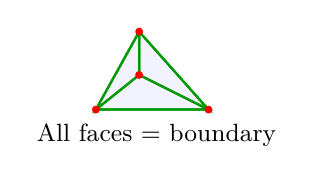
\begin{tikzpicture}[scale=1.1]
\coordinate (A) at (0,0);
\coordinate (B) at (1.3,0);
\coordinate (C) at (0.5,0.9);
\coordinate (D) at (0.5,0.4);

\fill[blue!8,opacity=0.6] (A)--(B)--(C)--cycle;
\draw[thick,green!60!black] (A)--(B)--(C)--cycle;
\draw[thick,green!60!black] (A)--(C)--(D)--cycle;
\draw[thick,green!60!black] (B)--(C)--(D)--cycle;
\draw[thick,green!60!black] (A)--(B)--(D)--cycle;
\foreach \p in {A,B,C,D}{\fill[red] (\p) circle (1.3pt);}
\node at (0.7,-0.3) {\small All faces = boundary};
\end{tikzpicture}
\end{center}
\end{columns}
\end{frame}

\begin{frame}{Example 5: Square Frame}

\begin{block}{Interpretation}
A 2D mesh with a hole has both interior and exterior boundaries.
The faces between inner and outer regions determine which edges are interior or boundary.
\end{block}


\begin{center}
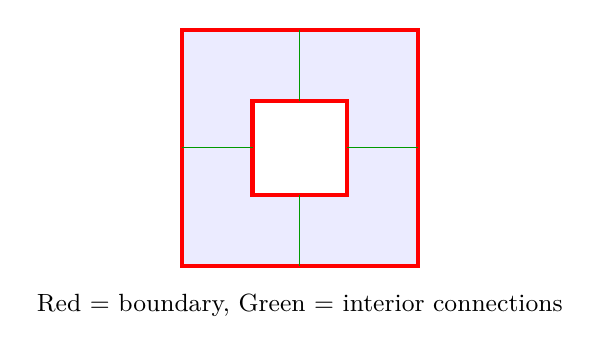
\begin{tikzpicture}[scale=1.0]
% outer square
\fill[blue!8] (-1.5,-1.5) rectangle (1.5,1.5);
% inner hole
\fill[white] (-0.6,-0.6) rectangle (0.6,0.6);
% outer boundary red
\draw[line width=1.5pt,red] (-1.5,-1.5)--(1.5,-1.5)--(1.5,1.5)--(-1.5,1.5)--cycle;
% inner boundary red
\draw[line width=1.5pt,red] (-0.6,-0.6)--(0.6,-0.6)--(0.6,0.6)--(-0.6,0.6)--cycle;
% a few interior connecting lines
\draw[thin,green!60!black] (-1.5,0)--(-0.6,0);
\draw[thin,green!60!black] (1.5,0)--(0.6,0);
\draw[thin,green!60!black] (0,-1.5)--(0,-0.6);
\draw[thin,green!60!black] (0,1.5)--(0,0.6);
\node at (0,-2.0) {\small Red = boundary, Green = interior connections};
\end{tikzpicture}
\end{center}
\end{frame}


\begin{frame}{Compatible Relative Orientations}
\begin{block}{Definition (Compatibility)}
Let \(M\) be a \(D\)–mesh with property ($\ast$). A relative orientation \(\epsilon\) is \emph{compatible} if every interior \((D\!-\!1)\)–cell \(c\) shared by \(D\)–cells \(a,b\) satisfies
\(\epsilon(a,c)=-\epsilon(b,c)\).
\end{block}

\begin{center}
% Square + Triangle sharing an edge E0
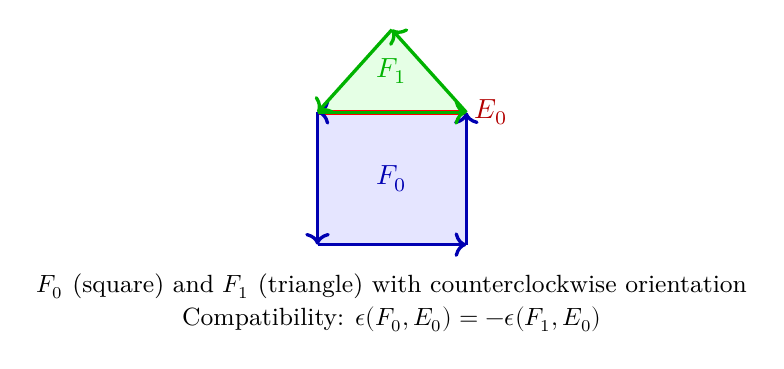
\begin{tikzpicture}[scale=1.05, dot/.style={circle,fill,inner sep=1.2pt}]
% Square coordinates
\coordinate (S1) at (0,0);
\coordinate (S2) at (1.8,0);
\coordinate (S3) at (1.8,1.6);
\coordinate (S4) at (0,1.6);
% Triangle sharing the top edge
\coordinate (T1) at (0,1.6);
\coordinate (T2) at (1.8,1.6);
\coordinate (T3) at (0.9,2.6);
% Draw faces
\fill[blue!10] (S1)--(S2)--(S3)--(S4)--cycle; % F0
\fill[green!10] (T1)--(T2)--(T3)--cycle;       % F1
% Face labels
\node[blue!70!black,font=\bfseries] at (0.9,0.8) {$F_0$};
\node[green!70!black,font=\bfseries] at (0.9,2.1) {$F_1$};
% Shared edge E0
\draw[line width=2pt,red] (S4)--(S3);
\node[red!70!black,font=\bfseries] at (2.1,1.6) {$E_0$};
% Oriented boundaries (counterclockwise) for faces
\draw[very thick,blue!70!black,->] (S1)--(S2);
\draw[very thick,blue!70!black,->] (S2)--(S3);
\draw[very thick,blue!70!black,->] (S3)--(S4);
\draw[very thick,blue!70!black,->] (S4)--(S1);
\draw[very thick,green!70!black,->] (T1)--(T2);
\draw[very thick,green!70!black,->] (T2)--(T3);
\draw[very thick,green!70!black,->] (T3)--(T1);
% Labels
\node at (0.9, -0.5) {\small $F_0$ (square) and $F_1$ (triangle) with counterclockwise orientation};
\node at (0.9, -0.9) {\small Compatibility: \(\epsilon(F_0,E_0)=-\epsilon(F_1,E_0)\)};
\end{tikzpicture}
\end{center}
\end{frame}


\begin{frame}{Boundary of a Combinatorial Mesh}

\begin{block}{Definition (Fundamental Class)}
Let \(M\) be a combinatorial mesh of dimension \(D\) satisfying property \((\ast)\),
and assume \(M\) admits a compatible relative orientation \(\epsilon\).
The \textbf{fundamental class} of \(M\) is defined as the formal sum of all \(D\)–cells:
\vspace{-0.3cm}
\begin{align*}
[M] \;=\; \sum_{a\in M_D} a \;\in\; C_D M.
\end{align*}
Intuitively, \([M]\) represents the entire oriented domain of the mesh.
If all orientations are consistent, opposite interior hyperfaces cancel in the boundary.
\end{block}
\end{frame}

\begin{frame}{Boundary of a Combinatorial Mesh}
\begin{block}{Boundary of the Fundamental Class}
Applying the boundary operator yields
\vspace{-0.3cm}
\begin{align*}
\partial[M]
&=\; \sum_{a\in M_D} \partial a
\;=\; \sum_{a\in M_D}\sum_{c\prec a,\,c\in M_{D-1}}\epsilon(a,c)\,c.
\end{align*}
For an \textbf{interior} hyperface \(c\), its two opposite contributions cancel:
\vspace{-0.3cm}
\begin{align*}
\epsilon(a_1,c)+\epsilon(a_2,c)=0,
\qquad (c\text{ shared by }a_1,a_2),
\end{align*}
while for a \textbf{boundary} hyperface (appearing in only one \(D\)–cell),
the term remains in \(\partial[M]\). Hence \(\partial[M]\) consists only of boundary elements.
\end{block}

\end{frame}


\begin{frame}{Example}
\vspace{-0.3cm}
\begin{block}{Setup and Fundamental Class}
Let \(M_2=\{F_0,F_1\}\) be two adjacent 2–cells (faces) of a planar mesh.
They share a common vertical edge \(E_0\).
Each face contributes its four oriented edges:
\vspace{-0.3cm}
\begin{align*}
[M] &= F_0 + F_1,\\
\partial[M] &= (E_1 + E_2 + E_3 + E_4 + E_5 + E_6),
\end{align*}
where the shared edge \(E_0\) cancels because it appears with opposite orientations in \(\partial F_0\) and \(\partial F_1\).
Thus, the mesh has one interior edge (\(E_0\)) and six boundary edges.
\end{block}

\vspace{-0.4cm}
\begin{center}
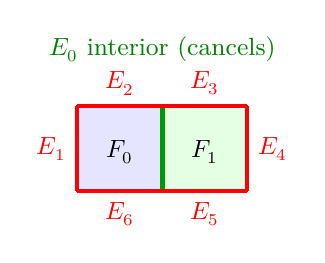
\begin{tikzpicture}[scale=0.9]
% --- Faces ---
\fill[blue!10] (0,0)--(1.2,0)--(1.2,1.2)--(0,1.2)--cycle; % Left face
\fill[green!10] (1.2,0)--(2.4,0)--(2.4,1.2)--(1.2,1.2)--cycle; % Right face

% --- Outlines ---
\draw[thick,black!70] (0,0)--(1.2,0)--(1.2,1.2)--(0,1.2)--cycle;
\draw[thick,black!70] (1.2,0)--(2.4,0)--(2.4,1.2)--(1.2,1.2)--cycle;

% --- Shared interior edge (green) ---
\draw[line width=1.6pt,green!60!black] (1.2,0)--(1.2,1.2);
\node[green!50!black] at (1.2,2.00) {\small $E_0$ interior (cancels)};

% --- Boundary edges (red) ---
\draw[line width=1.4pt,red] (0,0)--(0,1.2) node[midway,left] {\small $E_1$};
\draw[line width=1.4pt,red] (0,1.2)--(1.2,1.2) node[midway,above] {\small $E_2$};
\draw[line width=1.4pt,red] (1.2,1.2)--(2.4,1.2) node[midway,above] {\small $E_3$};
\draw[line width=1.4pt,red] (2.4,1.2)--(2.4,0) node[midway,right] {\small $E_4$};
\draw[line width=1.4pt,red] (2.4,0)--(1.2,0) node[midway,below] {\small $E_5$};
\draw[line width=1.4pt,red] (1.2,0)--(0,0) node[midway,below] {\small $E_6$};

% --- Face labels ---
\node at (0.6,0.55) {\small $F_0$};
\node at (1.8,0.55) {\small $F_1$};
\end{tikzpicture}
\end{center}
\end{frame}


\begin{frame}{Integration on Chains}
\vspace{-0.2cm}
\begin{block}{Definition}
For a top–degree cochain \(\sigma \in C^D M\),
the \textbf{integral} over the mesh is defined as its evaluation on the fundamental class:
\vspace{-0.3cm}
\begin{align*}
\int_M \sigma \;:=\; \sigma([M])
\;=\; \sum_{a\in M_D} \sigma(a).
\end{align*}
\end{block}

\vspace{-0.5cm}
\begin{block}{Example (Two–Square Mesh)}
\vspace{-0.5cm}
\begin{align*}
\int_M \sigma &= \sigma(F_0) + \sigma(F_1),\\
\int_{\partial M} \tau &= \tau(E_1) + \tau(E_2) + \tau(E_3) + \tau(E_4) + \tau(E_5) + \tau(E_6),
\end{align*}
where the shared interior edge \(E_0\) cancels out because of opposite orientation in both faces.
\end{block}
\end{frame}



\begin{frame}{de Rham Map, Fundamental Class}
\begin{block}{Remark (Smooth vs Discrete Integration)}
If \(X\) is a \(D\)–manifold and \(M\) is an embedded mesh via \(\varphi\), then for \(\omega\in\Omega^DX\):
\vspace{-0.3cm}
\begin{align*}
& (R_D\omega)(c)\;=\;\int_{\varphi(c)}\omega,\qquad c\in C_D M,\\
& \int_{\varphi(M)}\omega \;=\; (R_D\omega)([M]).
\end{align*}
\end{block}

\end{frame}

\begin{frame}{de Rham Map, Fundamental Class}
\vspace{-0.3cm}

\begin{block}{Two–Face Example Revisited}
Let \(M\) be the square–triangle complex from before, \([M]=F_0+F_1\).
\vspace{-0.3cm}
\begin{align*}
&(R_2\omega)(F_0) \;=\;\int_{\varphi(F_0)}\omega,\quad
(R_2\omega)(F_1) \;=\;\int_{\varphi(F_1)}\omega,\\
&(R_2\omega) \;=\; \big(\textstyle\int_{\varphi(F_0)}\omega\big)\,F^0
\;+\; \big(\textstyle\int_{\varphi(F_1)}\omega\big)\,F^1,\\[2pt]
&\int_{\varphi(M)}\omega
\;=\; (R_2\omega)([M])
\;=\; \big(\textstyle\int_{\varphi(F_0)}\omega\big)
\;+\; \big(\textstyle\int_{\varphi(F_1)}\omega\big).
\end{align*}
\end{block}

\vspace{-0.5cm}
\begin{center}
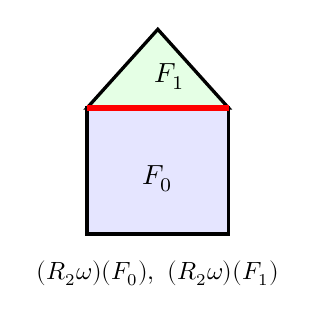
\begin{tikzpicture}[scale=1.0]
% Same geometry as Frame 3 (schematic)
\coordinate (S1) at (0,0);
\coordinate (S2) at (1.8,0);
\coordinate (S3) at (1.8,1.6);
\coordinate (S4) at (0,1.6);
\coordinate (T1) at (0,1.6);
\coordinate (T2) at (1.8,1.6);
\coordinate (T3) at (0.9,2.6);

\fill[blue!10] (S1)--(S2)--(S3)--(S4)--cycle; % F0
\fill[green!10] (T1)--(T2)--(T3)--cycle;       % F1

\draw[very thick] (S1)--(S2)--(S3)--(S4)--cycle;
\draw[very thick] (T1)--(T2)--(T3)--cycle;
\draw[line width=2pt,red] (S4)--(S3);

\node at (0.9,0.7) {$F_0$};
\node at (1.05,2.0) {$F_1$};

\node at (0.9,-0.5) {\small $(R_2\omega)(F_0),\ (R_2\omega)(F_1)$};
\end{tikzpicture}
\end{center}
\end{frame}

\begin{frame}{Discrete Cup Product on a CM}
\vspace{-0.3cm}
\begin{block}{Definition (Cup Product)}
Let \(M\) be a combinatorial mesh, \(D=\dim M\).
A bilinear map \(\smile:C^p M\times C^q M\to C^{p+q} M\) (for \(p,q\in\mathbb{N}\), \(p+q\le D\)) is a \textbf{cup product} if:
\vspace{-0.3cm}
\begin{align*}
&\textbf{(Graded commutativity)}\\
&\sigma\smile \rho \;=\; (-1)^{pq}\,\rho\smile \sigma,
\quad \sigma\in C^pM,\ \rho\in C^qM.\\[2pt]
&\textbf{(Graded Leibniz rule)}\\
&\delta(\sigma\smile\rho)\;=\; \delta\sigma\smile\rho \;+\; (-1)^p\,\sigma\smile\delta\rho.\\
&\textbf{(Locality)}\\
&\forall a\in M_{p+q}:\
(\sigma\smile\rho)(a)
=\sum_{\substack{b\preccurlyeq a,\ b\in M_p\\ c\preccurlyeq a,\ c\in M_q}}
\lambda_{a,b,c}\,\sigma(b)\,\rho(c)\quad(\lambda_{a,b,c}\in\mathbb{R}).\\[2pt]
&\textbf{(Unit)}\quad
\mathbb{1}\in C^0M,\ \ \mathbb{1}(N_i)=1\ \forall N_i\in M_0,\ \
\mathbb{1}\smile\sigma=\sigma\smile\mathbb{1}=\sigma.
\end{align*}
\end{block}
\end{frame}


\begin{frame}{\small{Forman Subdivision $\Rightarrow$ Quasi–Cubical Mesh}}
\begin{block}{Definition}
Let $M$ be a mesh with ``simple'' cells (no pathological vertices). The \emph{Forman subdivision} produces a mesh $K$ such that:
\begin{itemize}
    \item each $p$–cell of $M$ is subdivided into cells of $K$ that are topological $p$–cubes;
    \item incidence (face) relations are preserved and refined
    \item new vertices typically sit at cell barycenters / edge midpoints (schematic).
\end{itemize}

\end{block}
\end{frame}


\begin{frame}{Example (1D): Path $\rightarrow$ Subdivided Path}
\begin{block}{Original mesh $M$ (1D)}
\begin{center}
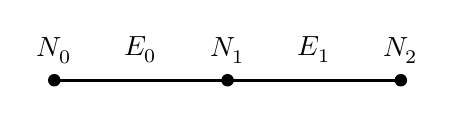
\begin{tikzpicture}[scale=1.1, dot/.style={circle,fill,inner sep=1.6pt}]
% vertices
\coordinate (A) at (0,0);
\coordinate (B) at (2.0,0);
\coordinate (C) at (4.0,0);
% edges
\draw[very thick] (A)--(B)--(C);
% nodes
\node[dot,label={$N_0$}] at (A) {};
\node[dot,label={$N_1$}] at (B) {};
\node[dot,label={$N_2$}] at (C) {};
% labels
\node at (1.0,0.35) {$E_0$};
\node at (3.0,0.35) {$E_1$};
\end{tikzpicture}
\end{center}
\end{block}

\begin{block}{Forman subdivision $K$ (1D)}

\begin{center}
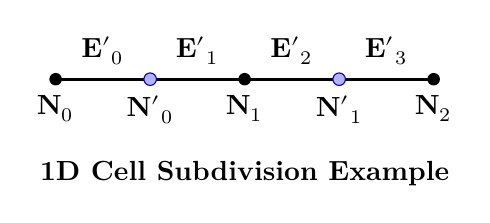
\begin{tikzpicture}[scale=1.2, dot/.style={circle,fill,inner sep=1.6pt}]
\coordinate (A) at (0,0);
\coordinate (B) at (2.0,0);
\coordinate (C) at (4.0,0);
\coordinate (M0) at (1.0,0);
\coordinate (M1) at (3.0,0);
\draw[very thick] (A)--(M0)--(B)--(M1)--(C);
\node[dot, fill=black, label=below:$\mathbf{N}_0$] at (A) {};
\node[dot, fill=black, label=below:$\mathbf{N}_1$] at (B) {};
\node[dot, fill=black, label=below:$\mathbf{N}_2$] at (C) {};
\node[dot, fill=blue!30, draw=blue!80!black, label=below:$\mathbf{N'}_0$] at (M0) {};
\node[dot, fill=blue!30, draw=blue!80!black, label=below:$\mathbf{N'}_1$] at (M1) {};
\node at (0.5,0.3) {$\mathbf{E'}_0$}; % Edge N0 -> N'0
\node at (1.5,0.3) {$\mathbf{E'}_1$}; % Edge N'0 -> N1
\node at (2.5,0.3) {$\mathbf{E'}_2$}; % Edge N1 -> N'1
\node at (3.5,0.3) {$\mathbf{E'}_3$}; % Edge N'1 -> N2
\node[font=\bfseries] at (2.0, -1.0) {1D Cell Subdivision Example};
\end{tikzpicture}
\end{center}
\end{block}
\end{frame}

\begin{frame}{\small{Example (2D): Pentagon $\rightarrow$ Quasi–Cubical Refinement}}
\vspace{-0.2cm}
\begin{block}{\small{Original mesh $M$ (2D)}}
\vspace{-0.3cm}
\begin{center}
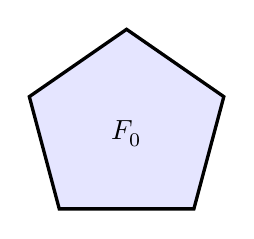
\begin{tikzpicture}[scale=0.95, dot/.style={circle,fill,inner sep=1.2pt}]
% pentagon vertices
\coordinate (P1) at (0,1.4);
\coordinate (P2) at (1.3,0.5);
\coordinate (P3) at (0.9,-1.0);
\coordinate (P4) at (-0.9,-1.0);
\coordinate (P5) at (-1.3,0.5);
% face
\fill[blue!10] (P1)--(P2)--(P3)--(P4)--(P5)--cycle;
\draw[very thick] (P1)--(P2)--(P3)--(P4)--(P5)--cycle;
% labels
\node at (0,0) {$\tiny F_0$};
\end{tikzpicture}
\end{center}
\end{block}

\vspace{-0.5cm}
\begin{block}{\small{Forman subdivision $K$ (2D, quasi–cubical cells)}}
\vspace{-0.4cm}
\begin{center}
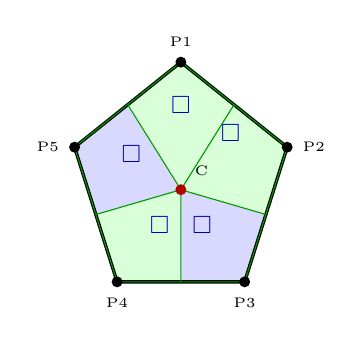
\begin{tikzpicture}[scale=0.9, dot/.style={circle,fill,inner sep=1.4pt}]

\coordinate (P1) at (0,1.8);
\coordinate (P2) at (1.5,0.6);
\coordinate (P3) at (0.9,-1.3);
\coordinate (P4) at (-0.9,-1.3);
\coordinate (P5) at (-1.5,0.6);
\coordinate (C) at (0,0); % Center

\coordinate (M12) at ($(P1)!0.5!(P2)$);
\coordinate (M23) at ($(P2)!0.5!(P3)$);
\coordinate (M34) at ($(P3)!0.5!(P4)$);
\coordinate (M45) at ($(P4)!0.5!(P5)$);
\coordinate (M51) at ($(P5)!0.5!(P1)$);

\fill[green!15] (C)--(M12)--(P2)--(M23)--cycle; % Quad 1
\fill[blue!15] (C)--(M23)--(P3)--(M34)--cycle;  % Quad 2
\fill[green!15] (C)--(M34)--(P4)--(M45)--cycle;
\fill[blue!15] (C)--(M45)--(P5)--(M51)--cycle;
\fill[green!15] (C)--(M51)--(P1)--(M12)--cycle;

\draw[very thick, black] (P1)--(P2)--(P3)--(P4)--(P5)--cycle;

\draw[thin, green!60!black] (M12)--(P2)--(M23);
\draw[thin, green!60!black] (M23)--(P3)--(M34);
\draw[thin, green!60!black] (M34)--(P4)--(M45);
\draw[thin, green!60!black] (M45)--(P5)--(M51);
\draw[thin, green!60!black] (M51)--(P1)--(M12);
\draw[thin, green!60!black] (C)--(M12) (C)--(M23) (C)--(M34) (C)--(M45) (C)--(M51);

\node[dot, label={above:\tiny P1}] at (P1) {};
\node[dot, label={right:\tiny P2}] at (P2) {};
\node[dot, label={below:\tiny P3}] at (P3) {};
\node[dot, label={below:\tiny P4}] at (P4) {};
\node[dot, label={left:\tiny P5}] at (P5) {};
\node[dot, fill=red!70!black, label={above right:\tiny C}] at (C) {}; % Center node

\node[scale=0.9, blue!70!black] at (0.7,0.8) {$\mathbf{\square}$};
\node[scale=0.9, blue!70!black] at (0.3,-0.5) {$\mathbf{\square}$};
\node[scale=0.9, blue!70!black] at (-0.3,-0.5) {$\mathbf{\square}$};
\node[scale=0.9, blue!70!black] at (-0.7,0.5) {$\mathbf{\square}$};
\node[scale=0.9, blue!70!black] at (0.0,1.2) {$\mathbf{\square}$};
\end{tikzpicture}
\vspace{-0.4cm}
\end{center}
\vspace{-0.4cm}
\end{block}
\vspace{-0.4cm}
\end{frame}


\begin{frame}{Example (3D): Tetrahedron and Cube}
\vspace{-0.2cm}
\begin{block}{Original $M$ (tetrahedron) and subdivision}
\begin{center}
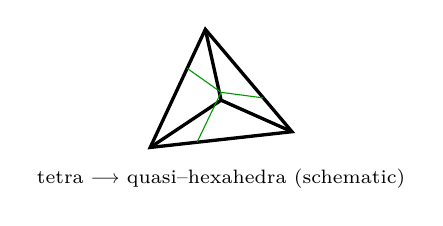
\begin{tikzpicture}[scale=1.0]
% Tetra outline (projection)
\coordinate (A) at (0,0);
\coordinate (B) at (1.8,0.2);
\coordinate (C) at (0.7,1.5);
\coordinate (D) at (0.9,0.6);
\draw[very thick] (A)--(B)--(C)--cycle;
\draw[very thick] (A)--(D)--(B);
\draw[very thick] (C)--(D);

\coordinate (BC) at (0.9,0.7);
\coordinate (F1) at ($(A)!0.33!(B)$);
\coordinate (F2) at ($(B)!0.33!(C)$);
\coordinate (F3) at ($(C)!0.33!(A)$);
\draw[thin,green!60!black] (BC)--(F1);
\draw[thin,green!60!black] (BC)--(F2);
\draw[thin,green!60!black] (BC)--(F3);

\node at (0.9,-0.4) {\scriptsize tetra $\longrightarrow$ quasi–hexahedra (schematic)};
\end{tikzpicture}
\end{center}
\end{block}
\vspace{-0.4cm}
\begin{block}{Cube $\rightarrow$ $2\times2\times2$ subcubes}
\begin{center}
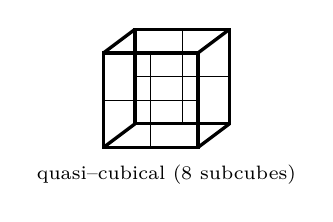
\begin{tikzpicture}[scale=1.0]
% front square
\draw[very thick] (0,0) rectangle (1.2,1.2);
% back square (shifted)
\draw[very thick] (0.4,0.3) rectangle (1.6,1.5);
% connectors
\draw[very thick] (0,0)--(0.4,0.3);
\draw[very thick] (1.2,0)--(1.6,0.3);
\draw[very thick] (1.2,1.2)--(1.6,1.5);
\draw[very thick] (0,1.2)--(0.4,1.5);
% inner $2\times2\times2$ grid on visible faces
\draw (0.6,0)--(0.6,1.2);
\draw (0,0.6)--(1.2,0.6);
\draw (1.0,0.3)--(1.0,1.5);
\draw (0.4,0.9)--(1.6,0.9);
% labels
\node at (0.8,-0.35) {\scriptsize quasi–cubical ($8$ subcubes)};
\end{tikzpicture}
\end{center}
\end{block}
\end{frame}

\begin{frame}{\small{Topological Orthogonality in a Quasi–Cubical Mesh}}
\vspace{-0.1cm}
\begin{block}{Definition (Orthogonality w.r.t.\ a Cell)}
Let \(K\) be a quasi–cubical mesh. For \(p,q\in\mathbb{N}\), \(a\in K_{p+q}\), \(b\in K_p\), \(c\in K_q\),
we write \((b,c)\in \perp_{p,q}(a)\) if \(b\subseteq a\), \(c\subseteq a\), and \(b\cap c=\{N\}\) is a \emph{single node}.
\end{block}

\begin{minipage}{.5\textwidth}
\begin{block}{\(F_0\)}
\begin{center}
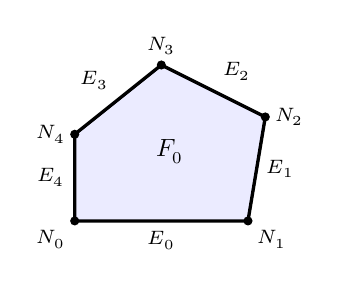
\begin{tikzpicture}[scale=1.1, dot/.style={circle,fill,inner sep=1.3pt}]
% Vertices
\coordinate (N0) at (0,0);
\coordinate (N1) at (2,0);
\coordinate (N2) at (2.2,1.2);
\coordinate (N3) at (1.0,1.8);
\coordinate (N4) at (0,1.0);

% Fill & outline
\fill[blue!8] (N0)--(N1)--(N2)--(N3)--(N4)--cycle;
\draw[very thick] (N0)--(N1)--(N2)--(N3)--(N4)--cycle;

% Label face
\node at (1.1,0.8) {\small $F_0$};

% Vertices
\foreach \i/\pos in {0/below left,1/below right,2/right,3/above,4/left}{
  \fill (N\i) circle (1.5pt) node[\pos] {\scriptsize $N_{\i}$};
}

% Edges
\draw[thick] (N0)--(N1) node[midway,below] {\scriptsize $E_0$};
\draw[thick] (N1)--(N2) node[midway,right] {\scriptsize $E_1$};
\draw[thick] (N2)--(N3) node[midway,above right] {\scriptsize $E_2$};
\draw[thick] (N3)--(N4) node[midway,above left] {\scriptsize $E_3$};
\draw[thick] (N4)--(N0) node[midway,left] {\scriptsize $E_4$};
\end{tikzpicture}
\end{center}
\end{block}
\end{minipage}%
\begin{minipage}{0.5\textwidth}
\begin{block}{\(F_1\)}
\begin{center}
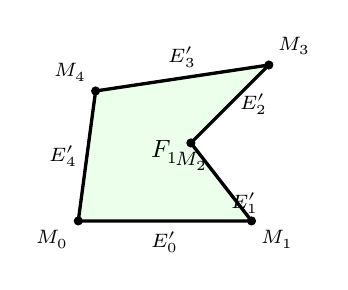
\begin{tikzpicture}[scale=1.1, dot/.style={circle,fill,inner sep=1.3pt}]
% Vertices (concave polygon)
\coordinate (M0) at (0,0);
\coordinate (M1) at (2,0);
\coordinate (M2) at (1.3,0.9);
\coordinate (M3) at (2.2,1.8);
\coordinate (M4) at (0.2,1.5);

\fill[green!8] (M0)--(M1)--(M2)--(M3)--(M4)--cycle;
\draw[very thick] (M0)--(M1)--(M2)--(M3)--(M4)--cycle;
\node at (1.0,0.8) {\small $F_1$};

\foreach \i/\pos in {0/below left,1/below right,2/below,3/above right,4/above left}{
  \fill (M\i) circle (1.5pt) node[\pos] {\scriptsize $M_{\i}$};
}

\draw[thick] (M0)--(M1) node[midway,below] {\scriptsize $E'_0$};
\draw[thick] (M1)--(M2) node[midway,below right] {\scriptsize $E'_1$};
\draw[thick] (M2)--(M3) node[midway,right] {\scriptsize $E'_2$};
\draw[thick] (M3)--(M4) node[midway,above] {\scriptsize $E'_3$};
\draw[thick] (M4)--(M0) node[midway,left] {\scriptsize $E'_4$};
\end{tikzpicture}
\end{center}
\end{block}
\end{minipage}
\end{frame}

\begin{frame}{Orthogonality Checks}
\vspace{-1.1cm}
\begin{align*}
&\text{\textbf{For Face \(F_0\)}}: (N_0,E_0)\in \perp_{0,1}(F_0):\ N_0,E_0\subset F_0,\ N_0\cap E_0=\{N_0\}.\\
&(N_0,E_1)\notin \perp:\ N_0\cap E_1=\emptyset.\\
&(N_0,F_0)\in \perp_{0,2}(F_0):\ N_0\cap F_0=\{N_0\}.\\
&(E_0,E_1)\in \perp_{1,1}(F_0):\ E_0\cap E_1=\{N_1\}.\\
&(E_0,E_0)\notin \perp:\ E_0\cap E_0=E_0.\\
&(E_1,E_1)\notin \perp:\ E_1\cap E_1=E_1.\\
&\text{\textbf{For Face \(F_1\)}}: (M_0,E'_0)\in \perp_{0,1}(F_1):\ M_0\cap E'_0=\{M_0\}.\\
&(M_0,E'_2)\notin \perp:\ M_0\cap E'_2=\emptyset.\\
&(M_2,E'_3)\in \perp_{1,1}(F_1):\ E'_2\cap E'_3=\{M_3\}.\\
&(E'_1,E'_3)\notin \perp:\ E'_1\cap E'_3=\emptyset.\\
&(E'_0,E'_4)\in \perp_{1,1}(F_1):\ E'_0\cap E'_4=\{M_0\}.\\
&(E'_2,E'_2)\notin \perp:\ E'_2\cap E'_2=E'_2.
\end{align*}
\end{frame}


\begin{frame}{Orthogonality on a Cube (3D Example)}
\vspace{-0.3cm}
Let \(a\) be the cube (3–cell). Then \((b,c)\in \perp_{p,q}(a)\) iff \(b,c\subseteq a\) and \(b\cap c=\{N\}\).
\vspace{-0.3cm}
\begin{align*}
&\perp_{0,1}(a):\ (V_i,E)\ \text{iff }V_i\in E.\\
&\perp_{0,2}(a):\ (V_i,F)\ \text{iff }V_i\in F.\\
&\perp_{1,2}(a):\ (E,F)\ \text{iff }E\subset F\ \text{and the intersection is its endpoint}.\\
&\perp_{1,1}(a):\ (E_1,E_2)\ \text{iff }E_1\cap E_2=\{V_k\}.\\
&\perp_{2,1}(a):\ (F,E)\ \text{iff }E\subset F\ \text{and }F\cap E=\{V_k\}.\\
&\text{Not orthogonal if intersection is an edge/face segment (not a node).}
\end{align*}
\vspace{-0.7cm}
\begin{center}
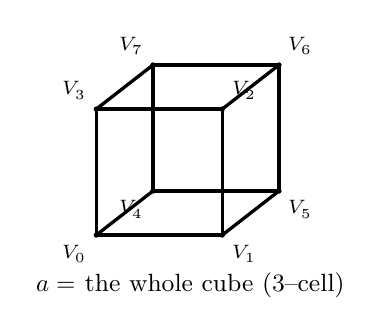
\begin{tikzpicture}[scale=0.8, dot/.style={circle,fill,inner sep=1.2pt}]

\coordinate (A) at (0,0);
\coordinate (B) at (2,0);
\coordinate (C) at (2,2);
\coordinate (D) at (0,2);
\coordinate (E) at (0.9,0.7);
\coordinate (F) at (2.9,0.7);
\coordinate (G) at (2.9,2.7);
\coordinate (H) at (0.9,2.7);
\draw[very thick] (A)--(B)--(C)--(D)--cycle;
\draw[very thick] (E)--(F)--(G)--(H)--cycle;
\draw[very thick] (A)--(E) (B)--(F) (C)--(G) (D)--(H);
\fill (A) circle (1.2pt) node[below left]  {\scriptsize $V_0$};
\fill (B) circle (1.2pt) node[below right] {\scriptsize $V_1$};
\fill (C) circle (1.2pt) node[above right] {\scriptsize $V_2$};
\fill (D) circle (1.2pt) node[above left]  {\scriptsize $V_3$};
\fill (E) circle (1.2pt) node[below left]  {\scriptsize $V_4$};
\fill (F) circle (1.2pt) node[below right] {\scriptsize $V_5$};
\fill (G) circle (1.2pt) node[above right] {\scriptsize $V_6$};
\fill (H) circle (1.2pt) node[above left]  {\scriptsize $V_7$};
\node at (1.5,-0.8) {\small \(a=\) the whole cube (3–cell)};
\end{tikzpicture}
\end{center}
\end{frame}


\begin{frame}{Quasi–Cubical Mesh: Convexity}
\vspace{-0.3cm}
\begin{block}{Definition (Convex and Non–Convex Cells)}
Let \(K\) be a quasi–cubical mesh embedded in a manifold \(M\).
Each cell \(c \in K_p\) is a connected subset of \(M\) homeomorphic to a convex polytope in \(\mathbb{R}^p\).\\
A cell is \textbf{convex} $\iff\ \forall x,y\in c,\ [x,y]\subseteq c.$ A cell is \textbf{non–convex} $\iff\ \exists\,x,y\in c\ \text{such that}\ [x,y]\not\subseteq c.$\\

Convex cells behave regularly under embedding; non–convex ones may self–intersect or create internal cavities.
\end{block}
\vspace{-0.2cm}
\begin{minipage}{.5\textwidth}
\vspace{-0.5cm}
\begin{center}
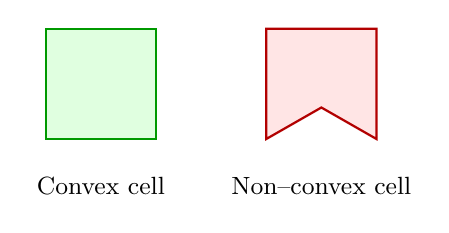
\begin{tikzpicture}[scale=1.0, dot/.style={circle,fill,inner sep=1.3pt}]
% Left: Convex cell (green square)
\fill[green!12,draw=green!60!black,thick] (-2.1,1.2) rectangle (-0.7,2.6);
\node at (-1.4,0.6) {\small Convex cell};

% Right: Non–convex cell (red concave pentagon)
\fill[red!10,draw=red!70!black,thick] (0.7,2.6)--(2.1,2.6)--(2.1,1.2)--(1.4,1.6)--(0.7,1.2)--cycle;
\node at (1.4,0.6) {\small Non–convex cell};
\end{tikzpicture}
\end{center}
\end{minipage}%
\begin{minipage}{.5\textwidth}
\textbf{Remark}: For a valid quasi–cubical mesh, all cells must be convex and their intersections must occur only along full shared faces. Non–convex cells violate this condition and break the orthogonality relations between subcells.
\end{minipage}%
\end{frame}


\begin{frame}{Embedding and Orientation Forms}
\vspace{-0.3cm}
\begin{block}{Definition}
Let \(K\) be a quasi–cubical mesh embedded in a manifold \(M\) by
\(\varphi: K \to \mathcal{P}(M)\), where \(\mathcal{P}(M)\) denotes subsets of \(M\).
Each \(p\)–cell \(c \in K_p\) carries an orientation form
\(\mathrm{or}_c \in \Omega^p\big(\varphi(c)\big)\) satisfying:
\vspace{-0.3cm}
\begin{align*}
&\text{(1) If } c \text{ is positively oriented, then } \mathrm{or}_c \text{ agrees with } \varphi.\\
&\text{(2) Reversing orientation of } c \text{ changes sign: } \mathrm{or}_{-c} = -\,\mathrm{or}_c.\\
&\text{(3) Forms are local representatives of geometric orientation in } M.
\end{align*}
\end{block}
\vspace{-0.3cm}
\hspace{-1.5cm}\begin{minipage}{.7\textwidth}
\begin{center}
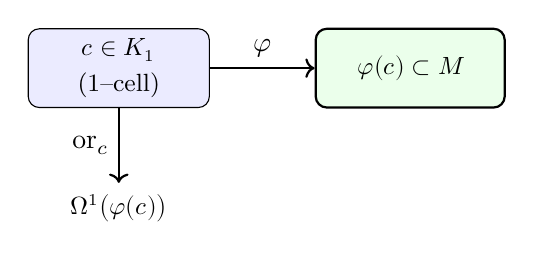
\begin{tikzpicture}[scale=0.95]
\node[draw,rounded corners,fill=blue!8,align=center,minimum width=2.3cm,minimum height=1.0cm,font=\small] (cell)
{ \(c\in K_1\) \\[2pt] (1–cell) };
\draw[->,thick] (cell.east) -- +(1.4,0)
node[midway,above] {\(\varphi\)}
node[right,draw,rounded corners,fill=green!8,align=center,minimum width=2.4cm,minimum height=1.0cm,font=\small]
{\(\varphi(c)\subset M\)};
\draw[->,thick] (cell.south) -- +(0,-1.0)
node[midway,left] {\(\mathrm{or}_c\)}
node[below,align=center,font=\small]
{\(\Omega^1\big(\varphi(c)\big)\)};
\end{tikzpicture}
\end{center}
\end{minipage}%
\hspace{-0.5cm}\begin{minipage}{.5\textwidth}
\begin{block}{Example}
For a 1–cell \(E_0\) embedded along the \(x\)–axis,
\(\mathrm{or}_{E_0} = dx\); reversing the orientation gives \(\mathrm{or}_{-E_0} = -dx.\)
\end{block}
\end{minipage}%
\end{frame}

\begin{frame}{Relative Orthogonal Orientation \(\epsilon^{\perp}\)}
\vspace{-0.3cm}
\begin{block}{Definition (Relative Orthogonal Orientation)}
Let \(K\) be quasi–cubical, \(p,q\in\mathbb{N}\), \(a\in K_{p+q}\), and \((b,c)\in \perp_{p,q}(a)\).
The \textbf{relative orthogonal orientation} \(\epsilon^{\perp}(a,b,c)\in\{-1,1\}\) is defined by
\vspace{-0.3cm}
\begin{align*}
\mathrm{or}_a \;=\; \epsilon^{\perp}(a,b,c)\, f\, \mathrm{or}_b \wedge \mathrm{or}_c,
\qquad f>0.
\end{align*}
\end{block}
\vspace{-0.5cm}
\begin{block}{Example in 2D (Square)}
Let a unit square face \(F_0\) with orientation \(\mathrm{or}_{F_0}=dx\wedge dy\).
Take two orthogonal edges at a common vertex:
\(\mathrm{or}_{E_0}=dx\) and \(\mathrm{or}_{E_1}=-dy\).
Then
\vspace{-0.3cm}
\begin{align*}
\mathrm{or}_{E_0}\wedge \mathrm{or}_{E_1}
&= dx \wedge (-dy) \;=\; -\,dx\wedge dy \;=\; -\,\mathrm{or}_{F_0},\\
\Rightarrow\quad \mathrm{or}_{F_0}
&= \epsilon^{\perp}(F_0,E_0,E_1)\, f \, \mathrm{or}_{E_0}\wedge \mathrm{or}_{E_1}
= \epsilon^{\perp}(F_0,E_0,E_1)\, f \, (-\,\mathrm{or}_{F_0}).
\end{align*}
As \(f>0\), we must have \(\epsilon^{\perp}(F_0,E_0,E_1)=-1\).
\end{block}
\end{frame}


\begin{frame}{3D Example (Cube) for \(\epsilon^{\perp}\)}
\vspace{-0.3cm}
\hspace{-1.2cm}\begin{minipage}{.5\textwidth}
\begin{center}
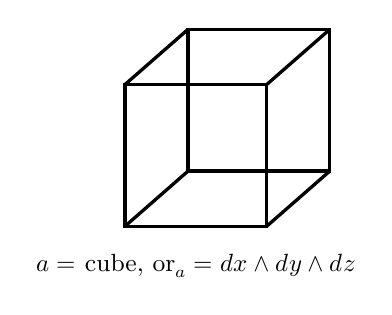
\begin{tikzpicture}[scale=1.0]
\coordinate (A) at (0,0);
\coordinate (B) at (1.8,0);
\coordinate (C) at (1.8,1.8);
\coordinate (D) at (0,1.8);
\coordinate (E) at (0.8,0.7);
\coordinate (F) at (2.6,0.7);
\coordinate (G) at (2.6,2.5);
\coordinate (H) at (0.8,2.5);
\draw[very thick] (A)--(B)--(C)--(D)--cycle;
\draw[very thick] (E)--(F)--(G)--(H)--cycle;
\draw[very thick] (A)--(E) (B)--(F) (C)--(G) (D)--(H);
\node at (0.9,-0.5) {\small \(a=\) cube, \(\mathrm{or}_a=dx\wedge dy\wedge dz\)};
\end{tikzpicture}
\end{center}
 \end{minipage}%
\begin{minipage}{.6\textwidth}
\begin{block}{Choice \((p,q)=(1,2)\)}
Pick an edge \(b\) parallel to \(x\) with \(\mathrm{or}_b=dx\), and a face \(c\) orthogonal to \(x\) with \(\mathrm{or}_c=dy\wedge dz\).
Then $\mathrm{or}_b\wedge \mathrm{or}_c = dx\wedge (dy\wedge dz) \;=\; dx\wedge dy\wedge dz \;=\; \mathrm{or}_a,\\
\Rightarrow\quad \epsilon^{\perp}(a,b,c)=+1.$ If instead \(\mathrm{or}_c=dz\wedge dy=-\,dy\wedge dz\), then \(\mathrm{or}_b\wedge \mathrm{or}_c= -\,\mathrm{or}_a\) and \(\epsilon^{\perp}(a,b,c)=-1\).
\end{block}
 \end{minipage}%
 \vspace{-0.3cm}
\begin{block}{Intrinsic View (Note)}
\(\epsilon^{\perp}\) can be defined intrinsically from relative orientations \(\epsilon\) and mesh topology \((\preccurlyeq)\), without explicit coordinates, by enforcing consistency with oriented incidence and \(\mathrm{or}_a \doteq \mathrm{or}_b\wedge \mathrm{or}_c\) at single–node intersections.
\end{block}
\end{frame}


\begin{frame}{Cup Product on Quasi-Cubical Mesh \(K\)}
\begin{block}{Definition (Orthogonality–Based Cup Product)}
For \(\sigma\in C^pK\), \(\rho\in C^qK\), \(a\in K_{p+q}\),
\vspace{-0.3cm}
\begin{align*}
(\sigma\smile \rho)(a)
\;=\;
\sum_{(b,c)\in \perp_{p,q}(a)}
\frac{\epsilon^{\perp}(a,b,c)\;\sigma(b)\;\rho(c)}{2^{\,p+q}}.
\end{align*}
\end{block}

\begin{block}{Theorem}
This definition satisfies the cup–product axioms:
graded commutativity, graded Leibniz rule with \(\delta\), locality, and the unit property.
\end{block}
\end{frame}


\begin{frame}{2D Square: Full Cup–Product Table}
\begin{block}{Square \(F_0\) with Counter-Clockwise (CCW) orientation}
Vertices \(N_0,N_1,N_2,N_3\) (CCW), edges:
\(\ E_0:N_0\to N_1\) (east),\\ \(\ E_1:N_1\to N_2\) (north),\\
\(\ E_2:N_2\to N_3\) (west),\\ \(\ E_3:N_3\to N_0\) (south).\\
Orientation forms:
\(\ \mathrm{or}_{F_0}=dx\wedge dy,\
\mathrm{or}_{E_0}=dx,\ \mathrm{or}_{E_1}=-dy,\
\mathrm{or}_{E_2}=-dx,\ \mathrm{or}_{E_3}=dy.\)
\end{block}
\vspace{-0.3cm}
\begin{block}{Case \((p,q)=(0,0)\) on a vertex \(a=N_i\)}
\vspace{-0.3cm}
\begin{align*}
(\sigma\smile\rho)(N_i)
&=\sum_{(b,c)\in \perp_{0,0}(N_i)} \epsilon^{\perp}(N_i,b,c)\,\sigma(b)\rho(c) \\
&=\epsilon^{\perp}(N_i,N_i,N_i)\,\sigma(N_i)\rho(N_i)
=\sigma(N_i)\rho(N_i).
\end{align*}
\end{block}
\end{frame}

\begin{frame}{2D Square: Full Cup–Product Table}
\begin{block}{Case \((p,q)=(1,0)\) on an edge \(a=E_j\)}
Pairs \((b,c)\in \perp_{1,0}(E_j)\) are \((E_j,N_\ell)\) with \(N_\ell\) an endpoint of \(E_j\).
Since 0–forms act as positive scalars, \(\epsilon^{\perp}=+1\).
With the factor \(2^{-(1+0)}=\tfrac12\),
\vspace{-0.3cm}
\begin{align*}
(\sigma\smile\rho)(E_j)
&=\tfrac12\big(\sigma(E_j)\rho(N_{\text{start}})+\sigma(E_j)\rho(N_{\text{end}})\big)\\
&=\tfrac12\,\sigma(E_j)\big(\rho(N_{\text{start}})+\rho(N_{\text{end}})\big).
\end{align*}
\end{block}
\vspace{-0.3cm}
\begin{block}{Case \((p,q)=(0,1)\) on \(a=E_j\)}
By symmetry,
\vspace{-0.3cm}
\begin{align*}
(\sigma\smile\rho)(E_j)
&=\tfrac12\big(\sigma(N_{\text{start}})+\sigma(N_{\text{end}})\big)\,\rho(E_j).
\end{align*}
\end{block}
\end{frame}


\begin{frame}{2D Square: \((p,q)=(1,1)\) on the Face \(F_0\)}
\begin{block}{Orthogonal Edge Pairs inside \(F_0\)}
Orthogonal ordered pairs \((b,c)\in \perp_{1,1}(F_0)\) are the adjacent edges meeting at one vertex:
\((E_0,E_1), (E_1,E_2), (E_2,E_3), (E_3,E_0)\).
Using the chosen edge orientations,
\vspace{-0.3cm}
\begin{align*}
&\mathrm{or}_{E_0}\wedge \mathrm{or}_{E_1} = dx\wedge(-dy) = -\,\mathrm{or}_{F_0}\ \Rightarrow\ \epsilon^{\perp}(F_0,E_0,E_1)=-1,\\
&\mathrm{or}_{E_1}\wedge \mathrm{or}_{E_2} = (-dy)\wedge(-dx) = +\,dy\wedge dx = -\,\mathrm{or}_{F_0}\\ &\Rightarrow\ \epsilon^{\perp}(F_0,E_1,E_2)=-1,\\
&\mathrm{or}_{E_2}\wedge \mathrm{or}_{E_3} = (-dx)\wedge dy = -\,dx\wedge dy = -\,\mathrm{or}_{F_0}\\& \Rightarrow\ \epsilon^{\perp}(F_0,E_2,E_3)=-1,\\
&\mathrm{or}_{E_3}\wedge \mathrm{or}_{E_0} = dy\wedge dx = -\,\mathrm{or}_{F_0}\ \Rightarrow\ \epsilon^{\perp}(F_0,E_3,E_0)=-1.
\end{align*}
\end{block}

\end{frame}

\begin{frame}{2D Square: \((p,q)=(1,1)\) on the Face \(F_0\)}
\begin{block}{Cup Value on \(F_0\)}
With the factor \(2^{-(1+1)}=\tfrac14\),
\vspace{-0.3cm}
\begin{align*}
(\sigma\smile\rho)(F_0)
=&\frac{1}{4}\sum_{(b,c)\in \perp_{1,1}(F_0)} \epsilon^{\perp}(F_0,b,c)\,\sigma(b)\rho(c)\\
=&\frac{1}{4}\Big[-\,\sigma(E_0)\rho(E_1)\;-\;\sigma(E_1)\rho(E_2)\;-\;\sigma(E_2)\rho(E_3)\\ &-\;\sigma(E_3)\rho(E_0)\Big].
\end{align*}
\end{block}
\end{frame}




\begin{frame}{Riemannian Mesh (RM): Measures}

\begin{block}{Definition}
A \emph{Riemannian mesh} is a combinatorial mesh \(M\) endowed with a cell–measure
\(\mu:M\to\mathbb{R}_{>0}\). If \(c\in M_p\) then \(\mu(c)\) has physical unit \(L^{p}\).

\textbf{Examples:} \(p{=}0\): dimensionless;\\ \(p{=}1\): length;\\ \(p{=}2\): area;\\ \(p{=}3\): volume).
\end{block}
\vspace{-0.3cm}
\begin{block}{Remark (Measure from an embedding)}
If $M$ is embeddable in a manifold $X$ (\(M\hookrightarrow X\)) via \(\varphi\), define
\vspace{-0.3cm}
\begin{align*}
\mu(c)=\int_{\varphi(c)}\mathrm{vol}_{\varphi(c)}.
\end{align*}
\end{block}
\end{frame}

\begin{frame}{RM - Example}
\vspace{-0.3cm}
\begin{block}{Example: Circle of radius \(r>0\)}
\begin{minipage}{.5\textwidth}
Mesh: two vertices \(N_0,N_1\) (antipodal), two edges (semicircles) \(E_0,E_1\), one face \(F_0\) (disk).
\end{minipage}%
\begin{minipage}{.5\textwidth}
\begin{center}
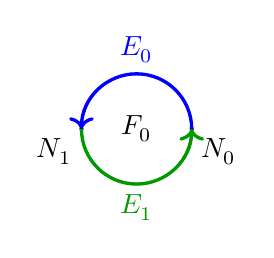
\begin{tikzpicture}[scale=0.5]
\draw[thick] (0,0) circle (1.4);
\fill (1.4,0) circle (1.5pt) node[below right] {$N_0$};
\fill (-1.4,0) circle (1.5pt) node[below left] {$N_1$};
\draw[very thick,blue,->] (1.4,0) arc (0:180:1.4) node[pos=0.5,above] {$E_0$};
\draw[very thick,green!60!black,->] (-1.4,0) arc (180:360:1.4) node[pos=0.5,below] {$E_1$};
\node at (0,0) {$F_0$};
\end{tikzpicture}
\end{center}
\end{minipage}%
\end{block}

\vspace{-0.3cm}
\begin{block}{Measures from the embedding in \(\mathbb{R}^2\)}
For radius \(r\) and circle/disk embedding,
\vspace{-0.3cm}
\begin{align*}
\mu(N_0)&=\mu(N_1)=1 \quad(\text{dimensionless convention}),\\
\mu(E_0)&=\mu(E_1)=\pi r \quad(\text{arc length}),\\
\mu(F_0)&=\pi r^2 \quad(\text{area}).
\end{align*}
(Any other fixed convention for \(\mu(N_i)\) is acceptable; we take \(1\).)
\end{block}

\end{frame}



\begin{frame}{A Particular Inner Product on an RM}
\begin{block}{Definition (Orthogonality–weighted diagonal product)}
Let \((K,\mu)\) be an RM of top dimension \(D\).
For \(p=0,1,\dots,D\) set \(\langle a^\bullet,b^\bullet\rangle_p=0\) for \(a\neq b\).
For a basis \(p\)–cochain \(c^\bullet\) (dual to \(c\in K_p\)),
\vspace{-0.3cm}
\begin{align*}
\big\langle c^\bullet,c^\bullet\big\rangle_p
=\frac{1}{2^{D}\,\mu(c)}
\sum_{\substack{a\in K_D\\ (b,c)\in \perp_{D-p,p}(a)}} \mu(a).
\end{align*}
Here \((b,c)\in\perp_{D-p,p}(a)\) means \(b\in K_{D-p},\,c\in K_p\) are topologically orthogonal inside \(a\).
\end{block}
\end{frame}

\begin{frame}{A Particular Inner Product on an RM}
\vspace{-0.2cm}
\begin{block}{Example: Four unit squares meeting at a vertex}
\vspace{-0.1cm}
\begin{minipage}{.5\textwidth}
\begin{center}
\includegraphics{build/lecture-15-2d-mesh.pdf}
\end{center}
\end{minipage}%
\begin{minipage}{.5\textwidth}
Take unit squares: \(\mu(F_i)=1\). Let edge lengths be \(\ell(E)=1\Rightarrow \mu(E)=1\), and \(\mu(N)=1\).
\end{minipage}%
\end{block}
\vspace{-0.4cm}
\begin{block}{\small{Computed weights (with \(D=2\))}}
\begin{minipage}{.7\textwidth}
\vspace{-0.4cm}
\begin{align*}
\langle N_0^\bullet,N_0^\bullet\rangle_0
&=\frac{1}{2^2\cdot 1}\sum_{i=1}^{4}\mu(F_i)=\tfrac{1}{4}\cdot 4=1,\\
\langle E^\bullet,E^\bullet\rangle_1
&=\frac{1}{2^2\cdot \mu(E)}\!\!\sum_{F\succ E}\!\mu(F)
=\frac{1}{4}\cdot\frac{2}{1}=\tfrac{1}{2},\\
\langle F^\bullet,F^\bullet\rangle_2
&=\frac{1}{2^2\cdot \mu(F)}\!\!\sum_{N\prec F}\!\mu(F)
=\frac{1}{4}\cdot\frac{4}{1}=1.
\end{align*}
\end{minipage}%
\begin{minipage}{.4\textwidth}
Thus the inner product\\ is diagonal with entries\\ \(1\) (vertices/faces) and\\ \(1/2\) (edges).
\end{minipage}%
\end{block}
\end{frame}

\begin{frame}{Discrete Hodge Stars}
\begin{block}{Definition}
For a compactly oriented RM \((K,\mu)\) with fundamental class \([K]\), the
\(\star_p:C^pK\to C^{D-p}K\) is the unique linear map such that for
all \(\pi\in C^pK\) and \(\rho\in C^{D-p}K\),
\vspace{-0.3cm}
\begin{align*}
\big\langle \star_p \pi,\ \rho\big\rangle_{D-p} \;=\; (\pi\smile \rho)[K].
\end{align*}
\end{block}

\begin{block}{Local formula (orthogonality form)}
If \(p=0,1,\dots,D\), \(\sigma\in C^pK\), \(c\in K_{D-p}\) (with dual \(c^\bullet\)),
\vspace{-0.3cm}
\begin{align*}
\big(\star_p\sigma\big)(c^\bullet)
=\frac{1}{2^{D}\,\langle c^\bullet,c^\bullet\rangle_{D-p}}
\sum_{\substack{a\in K_D,\, b\in K_{p}\\ (b,c)\in \perp_{p,D-p}(a)}}
\epsilon^{\perp}(a,b,c)\,\sigma(b^\bullet).
\end{align*}
\end{block}
\end{frame}

\begin{frame}{Example}
    \begin{block}{Explicit computation on the 4–square cross (with \(\mu=1\))}
Let \(D{=}2\).
\vspace{-0.3cm}
\begin{align*}
\star_0 N_0^\bullet
&=\tfrac{1}{2^{2}\langle F^\bullet,F^\bullet\rangle_2}\!\!\sum_{F\succ N_0}\!\epsilon^{\perp}(F,N_0,F)\,F^\bullet
=\tfrac{1}{4\cdot 1}\big(F_1^\bullet\!+\!F_2^\bullet\!+\!F_3^\bullet\!+\!F_4^\bullet\big),\\
\star_1 E_a^\bullet
&=\tfrac{1}{4\cdot \langle E^\bullet,E^\bullet\rangle_1}
\!\!\sum_{\substack{F\succ E_a\\ E'\perp E_a\text{ in }F}}\!\!\epsilon^{\perp}(F,E',E_a)\,E'^\bullet
=\tfrac{1}{4\cdot (1/2)}\big(\pm E_c^\bullet \pm E_d^\bullet\big)\\
&=\tfrac{1}{2}\big(\pm E_c^\bullet \pm E_d^\bullet\big),\\
\star_2 F_1^\bullet
&=\tfrac{1}{4\cdot \langle N^\bullet,N^\bullet\rangle_0}
\sum_{N\prec F_1}\epsilon^{\perp}(F_1,N,F_1)\,N^\bullet\\
&=\tfrac{1}{4}\big(N_{00}^\bullet+N_{01}^\bullet+N_{10}^\bullet+N_{11}^\bullet\big).
\end{align*}
Signs \(\epsilon^{\perp}\) follow the oriented edge/face conventions; with a consistent CCW choice, all shown coefficients are \(+\) as written.
\end{block}
\end{frame}

\begin{frame}{Adjoint Coboundaries \(\delta^*\)}
\begin{block}{Definition}
For the subspace of cochains with zero boundary trace \(\overline{C}^{\,p}K\),
the adjoint \(\delta_{p}^{*}:\overline{C}^{\,p}K\to \overline{C}^{\,p-1}K\) is characterized by
\vspace{-0.3cm}
\begin{align*}
\big\langle \delta_{p}^{*}\sigma,\ \eta\big\rangle_{p-1}
\;=\;
\big\langle \sigma,\ \delta_{p-1}\eta\big\rangle_{p},
\qquad
\sigma\in \overline{C}^{\,p}K,\ \eta\in \overline{C}^{\,p-1}K.
\end{align*}
\end{block}

\begin{block}{Interior stencil (local formula)}
If \(b\in K_{p-1}\) is interior,
\vspace{-0.3cm}
\begin{align*}
\big(\delta_{p}^{*}\sigma\big)(b^\bullet)
=\frac{1}{\langle b^\bullet,b^\bullet\rangle_{p-1}}
\sum_{\substack{a\succ b\\ a\in K_{p}}}
\epsilon(a,b)\ \langle a^\bullet,a^\bullet\rangle_{p}\ \sigma(a^\bullet).
\end{align*}
\end{block}
\end{frame}

\begin{frame}{Example}
    \begin{block}{Example on the 4–square cross (with \(\mu=1\))}
For \(D{=}2\) and the weights found earlier:
\vspace{-0.3cm}
\begin{align*}
(\delta_1^{*}\rho)(N_0^\bullet)
&=\frac{1}{\langle N_0^\bullet,N_0^\bullet\rangle_0}
\sum_{E\succ N_0}\epsilon(E,N_0)\,\langle E^\bullet,E^\bullet\rangle_1\,\rho(E^\bullet)\\
&=\sum_{E\succ N_0}\tfrac{1}{2}\,\epsilon(E,N_0)\,\rho(E^\bullet),\\
(\delta_2^{*}\phi)(E_a^\bullet)
&=\frac{1}{\langle E_a^\bullet,E_a^\bullet\rangle_1}
\sum_{F\succ E_a}\epsilon(F,E_a)\,\langle F^\bullet,F^\bullet\rangle_2\,\phi(F^\bullet)\\
&=2\sum_{F\succ E_a}\epsilon(F,E_a)\,\phi(F^\bullet).
\end{align*}
(Here \(\epsilon\) is the oriented incidence sign; the factors \(1/2\) and \(2\) arise from the diagonal inner products.)
\end{block}
\end{frame}

\begin{frame}{Discrete Identities and Comparison with the Smooth Case}
\begin{block}{Proposition (Discrete \(\delta^*\)–\(\star\) relation)}
For a compact oriented RM of top dimension \(D\) and \(p=0,\dots,D-1\),
\vspace{-0.3cm}
\begin{align*}
\delta_{D-p}^{*}\circ \star_p \;=\; (-1)^{p+1}\,\star_{p+1}\circ \delta_p,
\end{align*}
where \(\delta_p:C^pK\to C^{p+1}K\) is the discrete coboundary, \(\delta_{D-p}^{*}\) is its adjoint with respect to the RM inner products, and \(\star_q\) are the discrete Hodge stars.
\end{block}
\end{frame}

\begin{frame}{Summary of Exterior calculus and Combinatorial mesh calculus}
\vspace{-0.3cm}
\begin{center}
\resizebox{\textwidth}{!}{%
\begin{tabular}{|l|c|c||c||l|c|c|}
\hline
\multicolumn{3}{|c||}{\textbf{Exterior calculus}} & \textbf{Correspondence} & \multicolumn{3}{c|}{\textbf{Combinatorial mesh calculus}} \\
\hline
\textbf{Quantity/Operator} & \textbf{Expression} & \textbf{Dimension} & & \textbf{Quantity/Operator} & \textbf{Expression} & \textbf{Dimension} \\
\hline
Manifold & $M$ & 1 & Exact & Mesh & $\mathcal{M}$ & 1 \\
\hline
Submanifold & $V$ & 1 & Exact & Cell & $a$ & 1 \\
\hline
Vector field & $X$ & Generic & $-$ & $-$ & $-$ & $-$ \\
\hline
Differential form & $\omega$ & Generic & Exact & Cochain & $\sigma$ & Generic \\
\hline
Boundary & $\partial$ & 1 & Exact & Boundary operator & $\partial$ & 1 \\
\hline
Exterior derivative & $d$ & 1 & Exact & Coboundary operator & $\delta$ & 1 \\
\hline
Integration & $\int_M \omega$ & 1 & Exact & Discrete integration & $\sigma[\mathcal{M}]$ & 1 \\
\hline
Trace & $\mathrm{tr}\,\omega$ & 1 & Exact & Discrete trace & $\mathrm{tr}\,\sigma$ & 1 \\
\hline
Wedge product & $\wedge$ & 1 & Approximate & Cup product & $\smile$ & 1 \\
\hline
Metric tensor & $g_p^*$ & $\mathrm{L}^{-2p}$ & $-$ & $-$ & $-$ & $-$ \\
\hline
Inner product & $\langle\cdot,\cdot\rangle_p$ & $\mathrm{L}^{D-2p}$ & Approximate & Discrete inner product & $\langle\cdot,\cdot\rangle_p$ & $\mathrm{L}^{D-2p}$ \\
\hline
Hodge star & $\star_p$ & $\mathrm{L}^{D-2p}$ & Approximate & Discrete Hodge star & $\star_p$ & $\mathrm{L}^{D-2p}$ \\
\hline
Codifferential & $d_p^*$ & $\mathrm{L}^{-2}$ & Approximate & Adjoint coboundary operator & $\delta_p^*$ & $\mathrm{L}^{-2}$ \\
\hline
\end{tabular}%
}
\end{center}
\end{frame}


\begin{frame}[allowframebreaks]{Summary of Key Concepts} % The option must be in brackets here

\begin{itemize}
    \item The \textbf{cup product} on cochains is graded-commutative, local, and satisfies the \textbf{Leibniz rule} with $\delta$.
    \item \textbf{Forman subdivision} transforms a mesh $M$ into a quasi-cubical complex $K$ (where cells $\approx$ cubes).
    \item \textbf{Topological orthogonality} $(b,c) \in \perp_{p,q}(a)$ requires $b, c \subseteq a$ and $b \cap c = \{N\}$ (a single node).
    \item Examples in 2D/3D illustrate which pairs meet at exactly one vertex.
    \item Each cell $c$ carries an \textbf{orientation form} $\mathrm{or}_c$. For $(b,c) \in \perp_{p,q}(a)$, the orientation is:
          \[ \mathrm{or}_a = \epsilon^{\perp}(a,b,c)\,f\,\mathrm{or}_b \wedge \mathrm{or}_c \]
    \item The \textbf{orthogonality-based cup product} on $K$ is defined as:
          \[ (\sigma \smile \rho)(a) = \sum_{(b,c)\in\perp_{p,q}(a)} \frac{\epsilon^{\perp}(a,b,c)\,\sigma(b)\rho(c)}{2^{p+q}} \]
    \item All 2D cases for $(p,q)$ (e.g., (0,0), (1,0), (0,1), (1,1)) were computed explicitly with signs.
    \item \textbf{Cell measures} $\mu(\cdot)$ provide a \textbf{Riemannian metric} (RM); inner products are diagonal and local.
    \item The \textbf{discrete Hodge star} ($\star$) is defined via the cup product and $[K]$. Local formulas use $\perp$ and $\epsilon^{\perp}$.
    \item \textbf{Adjoint coboundaries} ($\delta^{*}$) yield divergence/flux-like stencils consistent with $\star$ and $\delta$.
    \item Signs and weights follow oriented incidence and the chosen metric (measures).
\end{itemize}
\end{frame}

\begin{frame}{Thanks}
  \cmcendframe
\end{frame}

\end{document}
